% Ubah judul dan label berikut sesuai dengan yang diinginkan.
\section{Tinjauan Pustaka}
\label{sec:tinjauanpustaka}

\subsection{Kursi Roda Elektrik}
Kursi roda adalah perangkat yang dioperasikan secara manual atau digerakkan dengan tenaga yang dirancang terutama untuk digunakan oleh individu dengan disabilitas mobilitas untuk tujuan utama bergerak di dalam ruangan, atau di dalam dan di luar ruangan.  Individu dengan disabilitas mobilitas harus diizinkan menggunakan kursi roda dan alat bantu mobilitas bertenaga manual, misalnya alat bantu jalan, kruk, tongkat, atau perangkat serupa lainnya yang dirancang untuk digunakan oleh individu dengan disabilitas mobilitas, di area mana pun yang terbuka untuk lalu lintas pejalan kaki \cite{ADA_2023}.

%Gambar 2.1
% Contoh input gambar
\begin{figure}[ht]
  \centering

  % Ubah dengan nama file gambar dan ukuran yang akan digunakan
  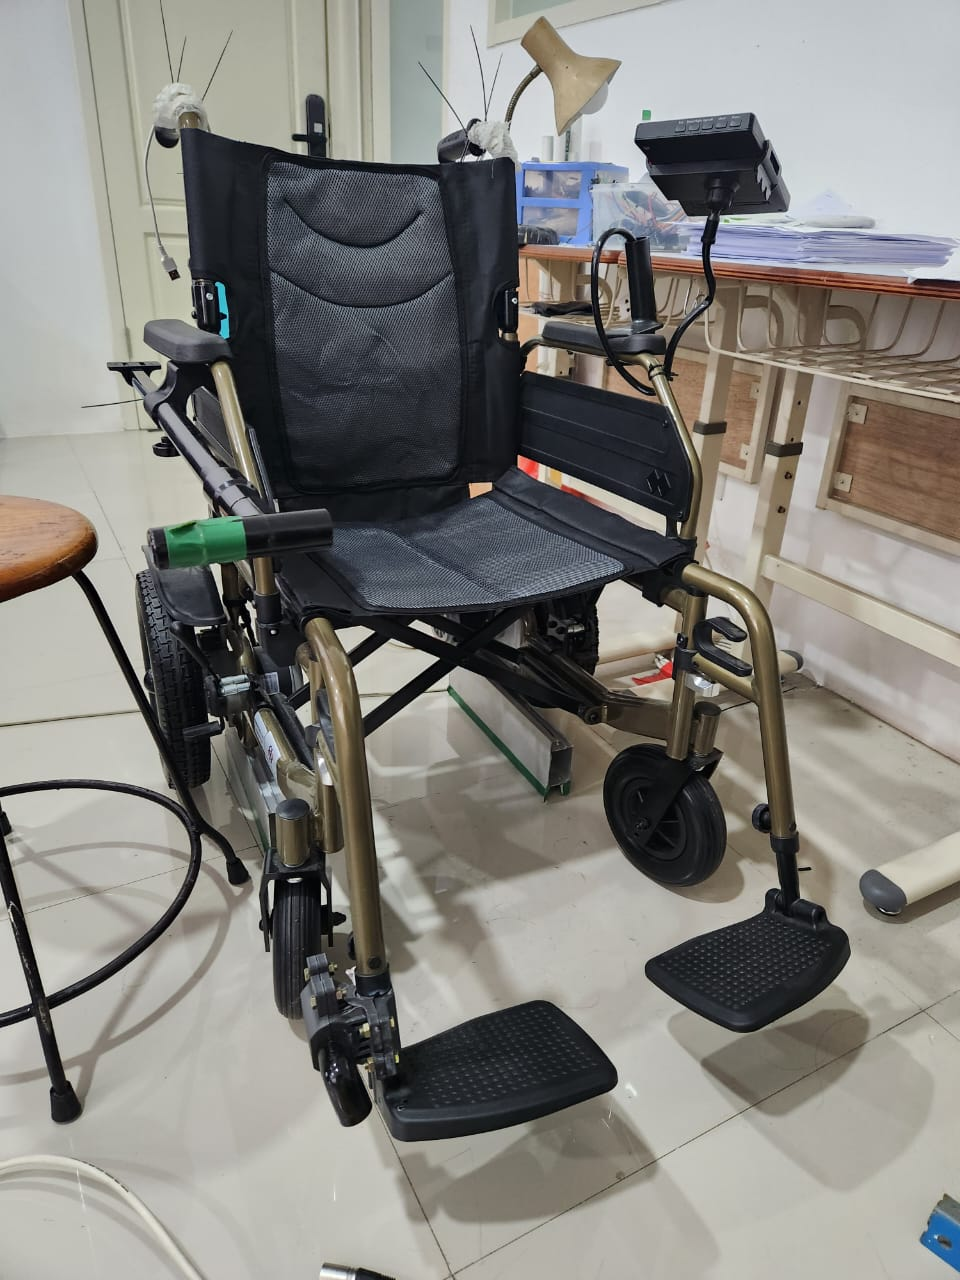
\includegraphics[scale=0.1]{gambar/bab3/kursi.jpeg}

  % Ubah dengan keterangan gambar yang diinginkan
  \caption{Kursi Roda Elektrik}
  \label{fig:kursiroda}
\end{figure}